\documentclass[portrait, a0, 30pt]{sciposter}
\usepackage[scaled=0.84]{helvet}
\usepackage{multicol, caption}
\usepackage[british]{babel}
\usepackage[utf8]{inputenc}
\usepackage{graphicx}
\usepackage{natbib}
\usepackage{times}
\usepackage{amsmath}
\usepackage{mathtools}
\usepackage{amsfonts}
\usepackage{verbatim}
\usepackage{graphicx}
\usepackage{framed}
\usepackage{xcolor}

\setcitestyle{authoryear,open={[},close={]}}

\DeclareMathOperator*{\argmax}{arg\,max}
\DeclareMathOperator*{\argmin}{arg\,min}

\DeclareMathOperator*{\KL}{{\rm KL}}
\DeclareMathOperator*{\const}{{\rm const}}

\colorlet{shadecolor}{lightgray!30}

\author{William van Rooij}
\title{Averaged Variational Inference for Hierarchical Modelling of Genetic Association}
\leftlogo{images/EPFL_logo}
\email{william.vanrooij@epfl.ch}
\date{July 2019}
\institute{École Polytechnique Fédérale de Lausanne, Lausanne, Switzerland}

\renewcommand{\titlesize}{\huge}
\renewcommand{\baselinestretch}{1.2}

\begin{document}
\maketitle
\begin{multicols*}{2}
\section{Introduction}
In \textbf{expression quantitative trait locus} (eQTL) studies, we estimate the association between \textbf{single nucleotide polymorphisms} (SNPs) and a gene expression phenotype, a \textbf{trait}. It is a \textit{small n, large p} situation where
\begin{itemize}
\item $n$ is the number of observations,
\item $p$ is the number of SNPs.
\end{itemize}
In a \textit{small n, large p} situation, the traditional methods such as \textbf{Markov Chain Monte Carlo} (MCMC) do not apply because of the cost of the computation being too large. As an alternative, we use \textbf{variational inference} from \citet{varInf}.

Moreover, the data is  highly correlated with a block structure, which complicates inference and interpretation. Here, we seek to enhance regression approaches in such difficult settings.



\section{Hierarchical Regression Model}
Let $\boldsymbol{X} = (X_1,\dots,X_p)$ represent the SNPs, and $\boldsymbol{y}$ represent the trait observed.

$\boldsymbol{y}$ is linearly related with the predictors $\boldsymbol{X}$ and has residual precision $\tau$. We suppose that they follow the following hierarchical model, for all $s = 1,\dots , p$ :
\begin{align*}
\boldsymbol{y} \mid \boldsymbol{\beta}, \tau &\sim\mathcal{N}\left(\boldsymbol{X\beta}, \tau^{-1}\boldsymbol{I}_n\right),\\
\beta_s \mid \gamma_s, \tau, \sigma^{-2} &\sim \gamma_s\;\mathcal{N} \left( 0, \sigma^2 \tau^{-1} \right) + (1-\gamma_s)\;\delta_0,\\
\gamma_s \mid \omega_s &\sim \mathrm{Bernoulli}\left(\omega_s\right),\\
\omega_s &\sim \mathrm{Beta}\left(a_s, b_s\right).
\end{align*}
where $\delta_0$ is the Dirac distribution, and $a_s$ and $b_s$ are chosen to enforce sparsity. $\boldsymbol{\gamma}$ is a binary matrix that that indicates which SNP is associated with the trait, i.e.,
\begin{center}
$\gamma_s = 1 \Longleftrightarrow$ SNP $ s $ is associated with the trait.
\end{center}
\section{Variational Inference}
Given a family of densities $\mathcal{D}$ over the parameters $\boldsymbol{\theta}$, variational inference approximates our density of interest $p(\boldsymbol{\theta}\mid\boldsymbol{y})$ by a distribution $q \in \mathcal{D}$ minimizing the ``reverse'' \textbf{Kullback--Leibler divergence}, by \citet{kl51},
\begin{equation*}
\KL (q \parallel p) = \int q(\boldsymbol{\theta}) \log \left\lbrace\frac{q(\boldsymbol{\theta})}{p(\boldsymbol{\theta}\mid\boldsymbol{y})}\right\rbrace.
\end{equation*}

We introduce the \textbf{evidence lower bound},
\[
\mathcal{L}(q)=\mathbb{E}_q\left[\log p(\boldsymbol{\theta},\boldsymbol{y})\right]-\mathbb{E}_q\left[\log q(\boldsymbol{\theta})\right] = \int q(\boldsymbol{\theta})\log\frac{p(\boldsymbol{y},\boldsymbol{\theta})}{q(\boldsymbol{\theta}}\mathrm{d}\boldsymbol{\theta},
\]
where $\mathbb{E}_q$ represents the expectation with respect to $q$.

The lower bound verifies
\[
\KL(q\parallel p) = \log(p)-\mathcal{L}(q).
\]

As the Kullbak--Leibler divergence can be difficult to minimize, variational inference maximizes the lower bound instead.

\begin{shaded}
When applied to highly correlated data, variational inference \textbf{underestimates} posterior variances, as explained in \citet{varInf}. \begin{itemize}
\item The lower bound $\mathcal{L}(q)$ tends to be \textbf{highly multimodal},
\item the mean-field independence assumption,
\item the reverse Kullback--Leibler divergence optimisation,
\end{itemize}
tend to concentrate mass on a single mode and neglect the rest.

To better handle the multimodality, we build a method consisting of averaging over multiple parameter initialisations with weights equal to the posterior model probability corresponding to the obtained mode, based on \citet{eff_inf}.
\end{shaded}
\section{Averaged LOCUS}
Assume that the data $\boldsymbol{y}$ has been obtained from a one of $K$ models $M_k,\quad k=1,\dots,K$. We want to estimate the association between the SNPs and the trait, i.e., we want to estimate $\boldsymbol{\gamma}$.

We perform a weighted average accounting for the likelihood that the data corresponds to each model. The more the model corresponds to the observed data, the more weight it will have in the average, i.e., for all $s = 1,\dots,p$, 
\begin{equation*}
\mathbb{E}\left[\gamma_s\mid \boldsymbol{y}\right] = \sum_{k=1}^K\mathbb{E}\left[\gamma_s\mid M_k, \boldsymbol{y}\right]\;p(M_k\mid \boldsymbol{y}).
\end{equation*}
The posterior probability for model $M_k$ is 
\begin{equation*}
p(M_k\mid \boldsymbol{y}) = \frac{p(\boldsymbol{y}\mid M_k)\;p(M_k)}{\sum_{j=1}^K p(\boldsymbol{y}\mid M_j)\; p(M_j)} \approx \frac{\mathcal{L}(q)\; p(M_k)}{\sum_{j=1}^K \mathcal{L}(q)\; p(M_j)}
\end{equation*}
where $p(\boldsymbol{y}\mid M_k)$ is the likelihood under model $M_k$, approximated by $\mathcal{L}(q)$, and $p(M_k)$ is the prior probability of model $M_k$.
\section{Performance}
We compare the performance of variable selection of five methods,
\begin{itemize}
\item classical variational inference ``LOCUS'',
\item averaged variational inference ``averaged LOCUS'',
\item their annealing augmented equivalents ``annealed LOCUS'' and ``averaged annealed LOCUS'',
\item averaged variational inference with equal weights ``averaged LOCUS (Equal weights)''
\end{itemize}

\begin{figure}[H]
\centering
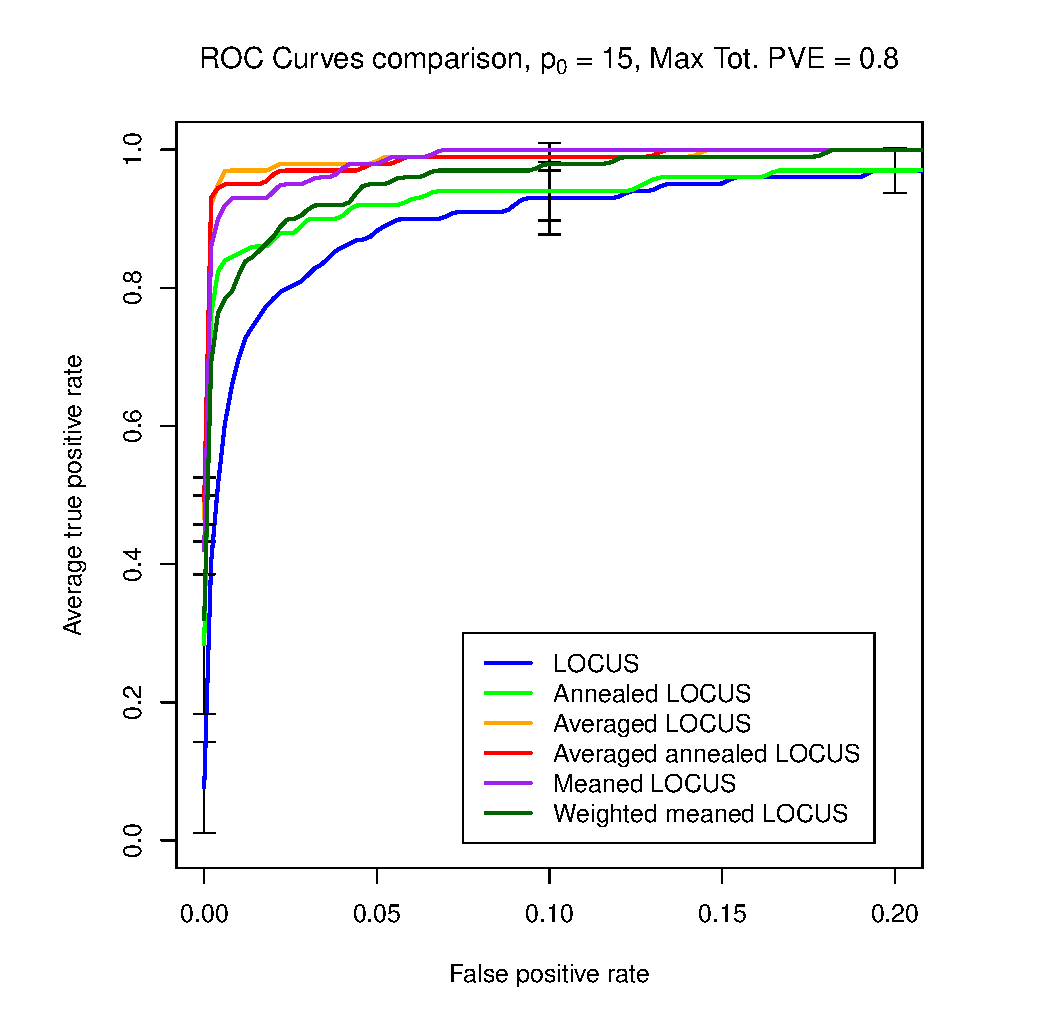
\includegraphics[width=9in]{images/ROC_curves.pdf}
\caption{\label{fig:ROC}Comparison of ROC curves between LOCUS, averaged LOCUS, their respective annealed versions, and averaged LOCUS with equal weights, colored in blue, orange, green, red, and purple respectively. The data involve $300$ observations, $15$ SNPs out of $500$ SNPs are associated with the trait. The response variance explained by the SNPs is below $80\%$.}
\end{figure}

The three averaging methods have similar variable selection performance, which is better than the standard LOCUS method's. The annealing step does not improve the performance of variable selection.
\section{Conclusion}
The averaged variational inference better handles the multimodality of the posterior and the shows the uncertainty due to the strong correlation structure in the data.

The averaged methods can be implemented in parallel, drastically diminishing the runtime. The runtime of the averaged annealing LOCUS is smaller than the runtime of averaged LOCUS.
\bibliography{references}
\bibliographystyle{apalike}
\end{multicols*}
\end{document}